
Le contenu des mini-jeux est très varié : jeu de rôle, jeu de gestion, jeu de plateforme, etc.
L'analyse des différences et des ressemblances entre ceux-ci, afin de définir ensuite une grammaire de description de jeux, est d'autant plus complexe.

Les difficultés d'implémentation des mini-jeux sont elles aussi différentes.
8 exemples concrets de jeux sont développés par la suite.
Cela permet d'appuyer l'analyse de ce que contient un mini-jeu.

Ces jeux n'ont pas été choisi par hasard : chacun possède un intérêt dans la description de ses règles et son implémentation. 

\note{tableau à vérifier}

\vspace{0.5cm}

\begin{tabular}{l|l}
 Jeu & Intérêt majeur \\
 \hline
 Pacman & Système de bonus \\
 1942 & Tirs \\
 Volley & Logique de score \\
 Course & Intelligence artificielle \\
 Mario & Niveaux \\
 Game\&Watch & Vague d'ennemis \\
 Billard & Collisions \\
 Gestion & Ressources \\
\end{tabular}

\vspace{0.5cm}

Tout d'abord, chaque jeu est présenté succintement, illustré par une capture d'écran d'une implémentation effectuée.
Dans un second temps, une analyse de leur contenu sera effectuée, appuyée par un tableau comparatif et les diagrammes UML de ces jeux.

\clearpage

\subsection{Présentation des mini-jeux}


\titlegame{Pacman}
\begin{minipage}{9cm}
Ce jeu est une adaptation du jeu classique de Pacman. 
Le joueur contrôle le Tux via les touches du clavier. 
Son but est de manger toutes les pommes sur le terrain tout en évitant les Microsoft qui essayent de l’attraper. 
Pour arriver à cet objectif, le joueur dispose de 3 vies. Le Tux peut manger des pommes en or pour pouvoir détruire les Microsoft pendant
une courte durée et marquer des points supplémentaires. Concernant l’affichage, le joueur voit le nombre de vies restantes, 
son score ainsi que le temps durant lequel les Microsoft restent vulnérables. Le jeu est adaptable car il est facile d’initialiser 
la carte à partir d’images et d’un fichier JSON.
\end{minipage}
\hfill
\begin{minipage}{6cm}
 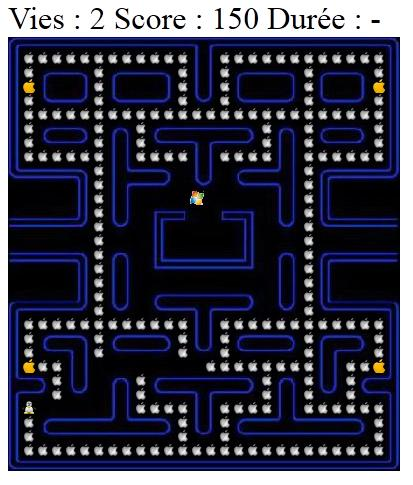
\includegraphics[width=\linewidth]{img/capturejeu_pacman}
\end{minipage}


\titlegame{1942}
\begin{minipage}{6cm}
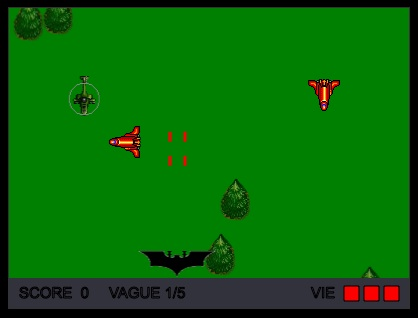
\includegraphics[width=\linewidth]{img/capturejeu_1942}
\end{minipage}
\hfill
\begin{minipage}{9cm}
Dans ce shoot them up (jeu d’action où le joueur fait face à une multitude d’ennemis), 
le joueur contrôle un vaisseau armé de deux canons pour détruire tous les véhicules adverses et gagner ainsi des points. 
Le joueur possède 3 vies pour faire le maximum de points. Lorsque le joueur perd une vie, il devient invincible durant une courte durée 
pour reprendre la main. Le vaisseau est contrôlé via le clavier. En ce qui concerne les ennemis, 
ils suivent des déplacements prédéfinis qui peuvent être paramétrés. 
Le joueur n’est pas obligé de tuer tous les ennemis mais le but est quand même de faire le plus grand score.
\end{minipage}

\titlegame{Volley}
\begin{minipage}{9cm}
CowCow volley party est un mini jeu humoristique mettant en scène deux vaches jouant au volley.
On peut jouer à ce jeu en mode solo contre une IA ou à deux joueurs. 
Le but est de remporter 2 sets, sachant que remporter un set revient à marquer \note{xxx} points. 
La vache dispose de 3 coups différents : passe courte, passe longue et un smash.
Les règles de ce jeu sont les mêmes que celles du volley classique.
La vache est contrôlée au clavier aussi bien en mode multijoueur qu’en mode solo.
\end{minipage}
\hfill
\begin{minipage}{6cm}
 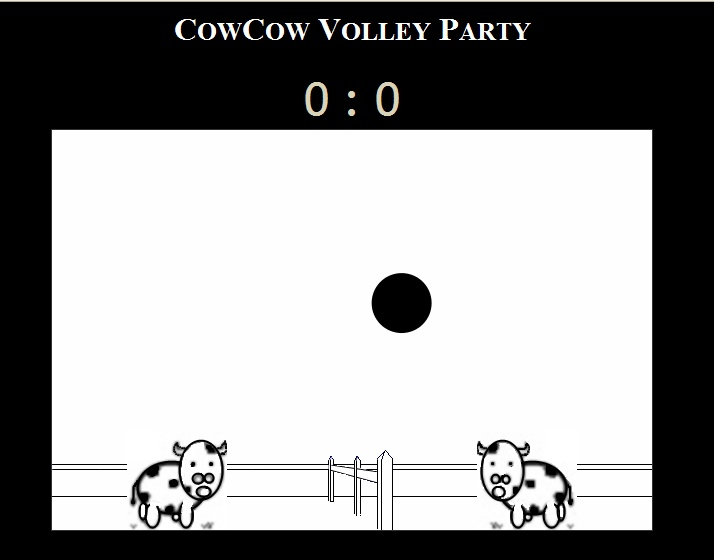
\includegraphics[width=\linewidth]{img/capturejeu_volleycowcow}
\end{minipage}


\titlegame{Course}
\begin{minipage}{6cm}
 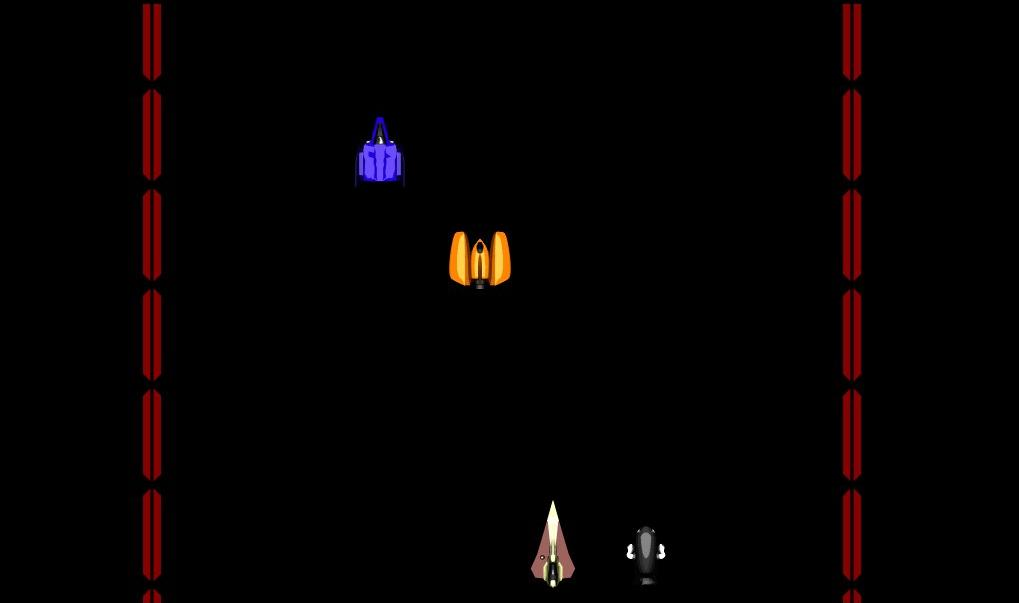
\includegraphics[width=\linewidth]{img/capturejeu_course}
\end{minipage}
\hfill
\begin{minipage}{9cm}
Ce jeu de course futuriste pour le web permet au joueur de se frotter à des intelligences artificielles pour faire le meilleur temps. 
Ce  n’est pas un jeu de course classique : en effet des bonus se trouvent sur le circuit :
un turbo, un bonus permettant d’augmenter le temps d’un des autres joueurs, un autre changeant la position d'un adversaire, etc. 
De plus, il existe différentes zones de circuit ayant des effets divers : inversion des commandes, changement de vitesses, etc.
Le joueur peut choisir son véhicule parmi une sélection de 12 vaisseaux différents. 
Le contrôle se fait au clavier. Ce jeu est adaptable : en effet, il est possible de créer facilement des circuits ainsi que des nouveaux bonus. 
Il serait aussi possible de mettre en place un système de lecture de fichier pour configurer les paramètres des différentes courses.
\end{minipage}

\titlegame{Mario}
\begin{minipage}{9cm}
Ce mini-jeu de plateforme reprend le principe des jeux du style de mario bros.
Un personnage, contrôlé au clavier et représenté par un rectangle, peut se déplacer sur les côtés ou sauter.
Il doit avancer au maximum, sans être touché par des ennemis, dessinés par des triangles, et sans tomber dans les trous du terrain.
Le personnage peut faire perdre des points de vie aux ennemis jusqu'à les tuer en leur sautant dessus. 
S'il les touche sur les côtés, il meurt et la partie est terminée.
La caméra avance lorsque le joueur avance suffisamment. Le joueur peut revenir à gauche jusqu'à la limite de l'écran.
Le terrain est généré aléatoirement et est infini.
Le but du jeu est d'obtenir le plus grand score. Le score diminue avec le temps et augmente lorsqu'un ennemi est tué ou que le personnage avance.
Il est facilement possible de changer le type de fonctionnement du jeu pour passer dans un mode où le but est de passer d'un niveau à un autre
avec des niveaux prédéfinis au préalable.
\end{minipage}
\hfill
\begin{minipage}{6cm}
 \framebox[\linewidth]{\parbox{\linewidth}{~ \vspace{4cm} Capture à venir ~\\~\\}}
\end{minipage}


\titlegame{Game \& Watch}
\begin{minipage}{6cm}
 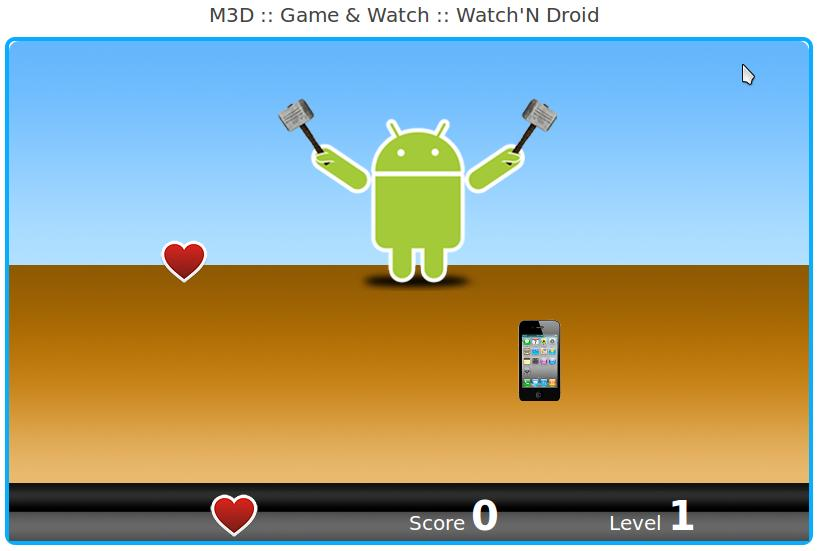
\includegraphics[width=\linewidth]{img/capturejeu_watchndroid}
\end{minipage}
\hfill
\begin{minipage}{9cm}
Watch’N’Droid est un mini-jeu du style Game \& Watch. 
Le joueur doit chasser ses ennemis avant que ces derniers ne l’atteignent. 
Les ennemis apparaissent un par un en bas de l’écran et montent pour atteindre le joueur à une certaine vitesse.
Cette dernière varie en fonction du niveau dans lequel le joueur se trouve. 
L’utilisateur est armé de deux marteaux pour détruire l’ennemi et donc marquer des points. 
Lorsque l’ennemi atteint le joueur se dernier perd une vie.
Lorsqu’il ne lui reste que deux vies, des vies bonus apparaissent sur l’écran et le joueur peut les ramasser. 
Lorsque le nombre de vie arrive à zéro, le joueur a la possibilité d’enregistrer son score si ce dernier fait partie
 des cinq meilleurs scores qui sont actuellement enregistrés.
\end{minipage}

\titlegame{Billard}
\begin{minipage}{9cm}
Ce mini-jeu de billard est un jeu multijoueurs en tour par tour. 
Il reprend les règles classiques du billard anglais (chaque joueur doit rentrer toutes les boules d’une couleur puis la noire). 
D’un point de vue gameplay, le joueur contrôle avec la souris la queue de billard. Cette dernière pointe automatiquement vers la boule blanche. 
Le joueur peut ainsi choisir l’angle avec lequel il compte frapper la boule blanche. En fonction du temps pendant lequel
 le joueur laisse le bouton de la souris enfoncé, le tir est plus ou moins fort. 
Pour l’affichage, chaque joueur voit le nombre de boules rentrées ainsi que sa couleur. 
Une icône verte apparait au niveau du joueur qui doit jouer. 
Le cadre bleu en bas de l’écran affiche la personne ayant gagné la partie !
\end{minipage}
\hfill
\begin{minipage}{6cm}
 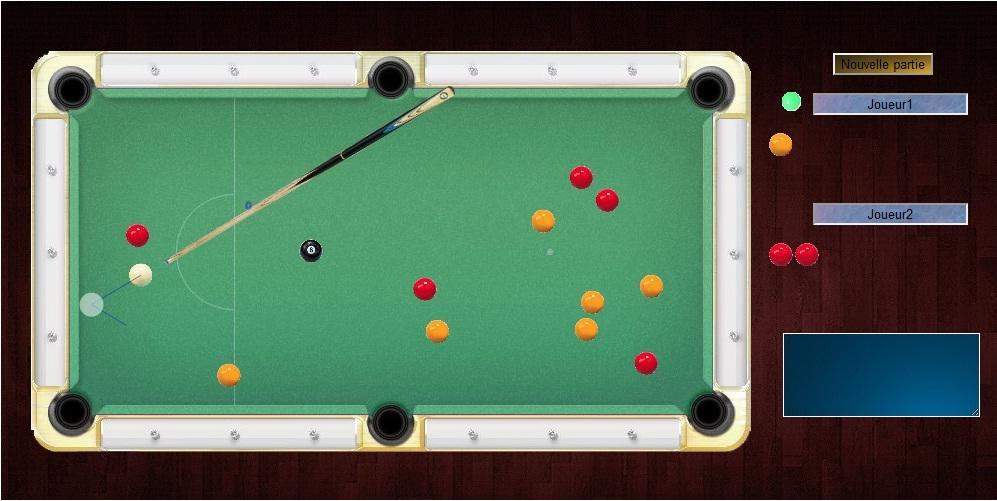
\includegraphics[width=\linewidth]{img/capturejeu_billard}
\end{minipage}


\titlegame{Gestion}
\begin{minipage}{6cm}
 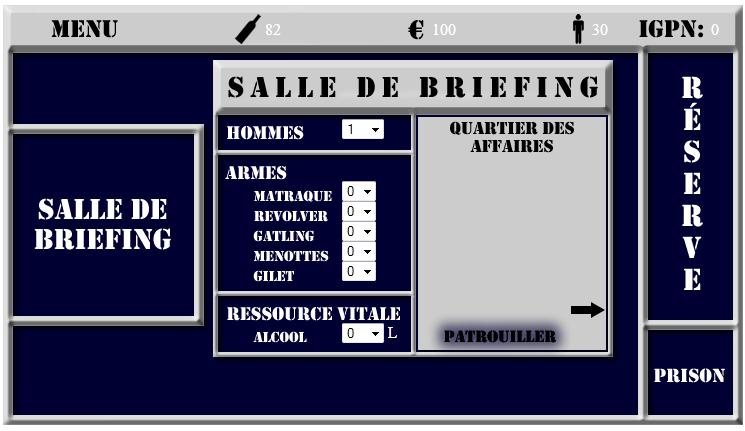
\includegraphics[width=\linewidth]{img/capturejeu_gestion2}
\end{minipage}
\hfill
\begin{minipage}{9cm}
Le jeu commissariat est un jeu de gestion du style Farmville. 
Le but est de maintenir et améliorer le commissariat en fonction des ressources disponibles.
Les ressources sont au nombre de quatre : le nombre de policiers, l’argent, l’indice IGPN et l’alcool. 
Il y a trois actions disponibles pour le joueur. Il peut envoyer des policiers en mission dans un quartier 
choisi pour ramener de l’argent ainsi qu’un prisonnier. Si un prisonnier est ramené, le joueur a la possibilité 
de libérer le prisonnier contre de l’argent ou de le tabasser (avec un fort risque de pénalité). 
Il peut aussi acheter des équipements ainsi que de l’alcool avec son argent. L’alcool est une ressource qui diminue constamment, 
le joueur doit veiller à toujours en avoir pour ne pas perdre. Il peut aussi perdre avec un indice d’IGPN trop élevé, cet indice 
monte avec toutes les mauvaises actions (tabasser un prisonnier, etc.).
\end{minipage}

\subsection{Comparaison des mini-jeux}

Ces mini-jeux ont été développés et leurs diagrammes UML sont disponibles en annexe.
De plus, ils permettent d'appuyer l'analyse de la description d'un mini-jeu.
Le tableau suivant récapitule les différents objectifs des jeux et leur style de terrain.

\vspace{0.5cm}
\noindent
\begin{tabular}{|l|| c|c|c|c|c|}
\hline
 Jeu &  Niveaux & Fin de niveau & Victoire & Score & Terrain \\
\hline
 Pacman & Oui & survie + tout ramassé & tous niveaux & Oui & Grille \\
\hline
 1942 & Oui & survie + ligne d'arrivée & tous niveaux & Oui & Progression verticale \\
\hline
 Volley &  Non & score & score & Oui & Plateau \\
\hline
 Course & Oui & survie + ligne d'arrivée & tous niveaux & Oui & Ruban \\
\hline
 Mario & Oui & survie + ligne d'arrivée & tous niveaux & Oui & Progression horizontale\\
\hline
 Game\&Watch & Oui & tout tué & tous niveaux & Oui  & Plateau et grille\\
\hline
 Billard & Non & toute boule rentrée & score & Oui & Plateau \\
\hline
 Gestion & Non & & & Oui & Grille\\
\hline
\end{tabular}

\vspace{0.5cm}

Le second tableau permet de comparer les aspects concernant le contrôle et les personnages.

\vspace{0.5cm}
\noindent
\begin{tabular}{|l|| c|c|c|c|}
\hline
 Jeu & Personnage & Contrôle & Autres actions & PNJ \footnote{Personnage non joué} \\
\hline
 Pacman &  Oui & direct via clavier & &  Oui \\
\hline
 1942 & Oui & direct via clavier & Tir & Oui  \\
\hline
 Volley & Oui & direct via clavier  & Tir, Saut & Oui \\
\hline
 Course & Oui & direct via clavier & Utilisation bonus & Oui \\
\hline
 Mario & Oui & direct via clavier &  Saut & Oui \\
\hline
 Game\&Watch & Oui & direct via clavier & Frappe & Oui  \\
\hline 
 Billard &  Oui {\small (si queue=joueur)} & direct via clavier & Force & Oui  \\
\hline
 Gestion &  Oui mais inutile & clic, sélection et action & Clic pour actions & Non \\
\hline
\end{tabular}

\vspace{0.5cm}

Ces tableaux permettent de mieux identifier les différences et points communs entre les différents jeux.

Par exemple, les objectifs au cours d'un niveau (ou pour un jeu sans niveau) se limitent souvent à atteindre une certaine zone
appelée ligne d'arrivée, ou éventuellement à remplir des conditions de temps ou de ressources. En effet, à la fois la vie et le score
peuvent être vus comme une ressource : il s'agit d'un état, et une condition sur celui-ci est nécessaire à la victoire.
En faisant des conjonctions et des disjonctions de ces différentes possiblités, il est possible de définir 
les conditions de victoire pour tous les jeux (sauf le jeu de gestion).

En revanche, si on regarde comment le monde est construit, il est très différent d'un jeu à l'autre.
Pour certains comme Pacman, il est défini par une grille, pour d'autres comme le jeu de course, il est défini via un ruban.

Le tableau permet de distinguer clairement le jeu de gestion des autres jeux.
La grammaire proposée par la suite ne prendra pas en compte ce type de jeux.
La comparaison se base donc sur les autres jeux, pour définir des concepts qui seront détaillés dans les parties suivantes.
Retirer du langage de description les jeux de gestion n'empêchent pas de couvrir un nombre important de jeux.
Il serait possible par exemple de définir plusieurs grammaires, chacune couvrant une catégorie de jeux afin de pouvoir
créer plusieurs types de jeux. Ainsi une autre grammaire pourrait spécialement être créee pour les jeux de gestion.
De la même façon, il est difficile de trouver des points communs entre les 7 mini-jeux restants et un jeu de rôle classique où le joueur
doit réaliser plusieurs quêtes.

\subsection{Analyse des mini-jeux}

On remarque tout d'abord que tous les mini-jeux possèdent une boucle de rafraîchissement.
Cette dernière permet à la fois d'effectuer les différentes actions telles que le déplacement des personnages non joueurs et de gérer 
les différents 'timer' du jeu.

Ensuite, dans les mini-jeux se retrouvent souvent la notion d'un avatar, petit personnage que le joueur peut déplacer.
Différentes actions peuvent se greffer à cet avatar selon les jeux, souvent le déplacement, le saut, le tir.
Cet avatar a des caractéristiques que l'on retrouve dans plusieurs jeux comme la vie, d'autres plus rares comme une quantité de points de magie.
De même, dans de nombreux jeux se trouvent la notion d'ennemis : des personnages non joués, dont le comportement est prédéfini.

De plus, la notion de ressources est très utile. Il s'agit d'une variable qui définit un état par exemple sur les entiers tel que le score.
Celle-ci peut être modifiée selon les évènements qu'il se passe dans le jeu.

Enfin, dans tous les mini-jeux, le concept de collision est très utile. Celle-ci cause la plupart du temps de nombreuses conséquences (mort d'ennemis, de joueurs,
incapacité de passer un obstacle, etc.)